\documentclass[openany]{book}
\input{notes_white}
\usepackage{mathtools}
\usepackage{circuitikz}
\settitle{The Mysteries of Recursion}
\begin{document}
\title{\Large{\underemphasise{Mathematical Foundations of Computer Science}} \\ \vspace{5pt}
\large{Series of Articles on Theoretical Computer Science}}
\author{Eklavya Raman \\ \vspace{5pt} (24MS, IISER Kolkata)} 
\date{\today}
\maketitle
\tableofcontents
\chapter{Article 1: The Mysteries of Recursion}
\section{Introduction}
All of you who have programmed before, know that many problems can be solved using basic loops like \texttt{for} and \texttt{while}. You might even think that are the only way to solve problems, or the most efficient in most cases. Now, what you think is true up to a certain extent, but what if I told you that any problem that you can make an algorithm for using a loop, can also be solved using recursion? Recursion is a beautiful concept, and it is the basis of many algorithms that you will see while solving all sorts of different problems. In this article, we will explore the concept of recursion, how it works, and why it is so powerful. I will also show you some examples of using recursion, and why it is so useful. 
\section{Every Algorithm is Recursive}
When most people start programming, they are taught to use conditional statements, basic arithmetic operators, loops and what not. They are taught to use these pre built tools, and for most intents and purposes, these tools are in fact sufficient for solving problems. However, there comes a time in every serious programmer's life that they encounter the dreaded concept of recursion.
\subsection{The Fibonacci Sequence, a Classic Example}
Most people are introduced to recursion through the classic example of the fibonacci sequence. I will not go into the details of the fibonacci sequence here, or trust me, we would be here for a long time. Anyhow, I think this is a fantastic example to introduce recursion for the following reasons: \\
\begin{enumerate}
    \item The definition of the sequence itself is easy to understand and implement. In fact, most people would be able to compute the first few terms of the sequence easily in their heads. 
    \item The sequence is extremely beautiful, and has a host of interesting and novel properties that one can readily observe if they choose to explore it in detail. 
\end{enumerate}
However, if you look at the most efficient "easy to learn" algorithm to compute the fibonacci sequence, it is actually just a simple loop: 
\begin{lstlisting}[language=Python]
def fibonacci(n):
    if n>0:
        a = 0 
        b = 1
        for i in range(1, n):
            a, b = b, a + b
        return b
\end{lstlisting}
This is a simple loop that computes the fibonacci sequence in \(\mathcal{O}(n)\) time (this basically means that the time taken to compute the \(n\)th term of the sequence is proportional to \(n\)). However, if you just look at the definition of the fibonacci sequence, and build an algorithm based on that, you will end up with a recursive algorithm that looks like this:
\begin{lstlisting}[language=Python]
    def fib(n):
        if n == 0:
            return 0 
        if n == 1:
            return 1
        else:
            return fib(n-1) + fib(n-2)
\end{lstlisting}
This is a simple recursive algorithm that computes the \(n\)th term of the fibonacci sequence. However, this algorithm is not efficient at all, and takes \(\mathcal{O}(2^n)\) time to compute the \(n\)th term of the sequence. To understand this better, let's look at the recursion tree for this algorithm. \\
\begin{figure}[!ht]
\centering
\resizebox{0.5\textwidth}{!}{%
\begin{circuitikz}
\tikzstyle{every node}=[font=\LARGE]
\draw[fill={rgb,255:red,255; green,255; blue,255}] (0.5,17.75) rectangle (16,2);
\draw  (10,16.75) rectangle  node {\LARGE fib(6)} (12.5,15.5);
\draw [->, >=Stealth] (11.25,15.5) -- (8.75,14.25);
\draw [->, >=Stealth] (11.25,15.5) -- (13.75,14.25);
\draw  (7.5,14.25) rectangle  node {\LARGE fib(5)} (10,13);
\draw  (12.5,14.25) rectangle  node {\LARGE fib(4)} (15,13);
\draw [->, >=Stealth] (8.75,13) -- (6.25,11.75);
\draw [->, >=Stealth] (8.75,13) -- (11.25,11.75);
\draw  (5,11.75) rectangle  node {\LARGE fib(4)} (7.5,10.5);
\draw  (10,11.75) rectangle  node {\LARGE fib(3)} (12.5,10.5);
\draw [->, >=Stealth] (6.25,10.5) -- (5,9.25);
\draw [->, >=Stealth] (6.25,10.5) -- (7.5,9.25);
\draw  (4.25,9.25) rectangle  node {\LARGE fib(3)} (5.75,8);
\draw  (6.75,9.25) rectangle  node {\LARGE fib(2)} (8.25,8);
\draw [->, >=Stealth] (5,8) -- (3.75,6.75);
\draw [->, >=Stealth] (5,8) -- (6.25,6.75);
\draw  (3,6.75) rectangle  node {\LARGE fib(2)} (4.5,5.5);
\draw  (5.5,6.75) rectangle  node {\LARGE fib(1)} (7,5.5);
\draw [->, >=Stealth] (3.75,5.5) -- (2.5,4.25);
\draw [->, >=Stealth] (3.75,5.5) -- (5,4.25);
\draw  (1.5,4.25) rectangle  node {\LARGE fib(1)} (3.5,3);
\draw  (4,4.25) rectangle  node {\LARGE fib(0)} (6,3);
\end{circuitikz}
}%

\label{fig:my_label}
\end{figure}
You will realise, that the recursion tree is binary, and the height of the tree is $n$. Then the number of nodes is $2^n$, and hence the time complexity of the algorithm is \(\mathcal{O}(2^n)\). This is a very inefficient algorithm, and it is not practical to use it for large values of \(n\). This algorithm also wastes a lot of memory (why?)\\
Looking at this algorithm, you might be inclined to think that recursion must be useless if it is inefficient. However, this is not the case in general. \\
To understand the significance of recursion, we need to go all the way back to the notion of an algorithm. 
\subsection{What is an Algorithm and how is it related to Recursion?}
The study of algorithms is fundamental to computer science, and offers applications in a wide range of fields, from artifical intelligence, cryptography, computational chemistry, biology and many more. The first problem we need to tackle is to find a satisfactory definition of an algorithm. \\ \\
Informally, we can define an algorithm as a sequence of instructions and rules that can be applied to a set of inputs to produce an output. This definition itself is very vague, and does not help us construct a theory of algorithms. There were certain people who tried to formalise this informal notion, so that a formal framework be constructed to solve problems in a systematic way. \\ \\
\underemphasise{Church and Turing} are two people who pioneered the study of algorithms. Their work led to the development of the field of Theoretical Computer Science, and the concept of computability. Their attempts at formalization of the notion of an algorithm in terms of functions, led to the discovery that a particular class of functions, that is \textbf{recursive functions}, are the mathematical analogues of algorithms, or the ones that match the best with our informal definition. \\ \\
Although we face a few problems, since the class of recursive functions is broader than the class of functions that can be computed by algorithms, we can still use the properties of recursive functions to study algorithms. \\ \\
The formal definition of recursive functions is beyond the scope of this article. In essence, recursive functions are functions that can be defined in terms of themselves. This is the essence of recursion, and it is what makes it so powerful. \\ \\
\textbf{And since the class of recursive functions is a superset of the class of functions that can be computed by algorithms, we can say that any algorithm can be expressed in terms of recursive functions. This is the essence of recursion, and it is what makes it so powerful.} 
\section{The Power of Recursion}
Now, since it is established that every algorithm can be expressed in terms of recursive functions (even basic mathematical operations like addition or comparison), we now have a way to solve problems that are not efficiently solvable using loops. This section will explore the power of recursion, and how it can be used to solve problems that are not efficiently solvable using loops. 
\subsection{The Sorting Problem}
One of the most common and important problems in computer science is coincidentally, one of the first problems that you might encounter in you programming journey: The Sorting Problem. Hell, you might even have solved it before. Here, we present 2 algorithms that solve the sorting problem, one using loops, and the other using recursion. \\ \\
The first is the insertion sort algorithm, which is a simple algorithm that sorts an array of numbers in ascending order. The algorithm works by iterating through the array, and inserting each element into its correct position in the sorted part of the array. The algorithm can be implemented using a simple loop, and has a time complexity of \(\mathcal{O}(n^2)\). Here is the implementation in Python:
\begin{lstlisting}[language=Python]
def insertion_sort(arr):
    for i in range(1, len(arr)):
        key = arr[i]
        j = i - 1
        while j >= 0 and key < arr[j]:
            arr[j + 1] = arr[j]
            j = j - 1
        arr[j + 1] = key
    return arr
\end{lstlisting}
Insertion sort is a simple but powerful algorithm, and often used in practice. It is easy to understand, and can be implemented in a few lines of code. However, it is not the most efficient algorithm for sorting large arrays. \\ \\
The second algorithm is the merge sort algorithm, which is more efficient when working with large arrays. The algorithm works by dividing the array into two halves, sorting each half recursively, and then merging the two sorted halves back together. The algorithm can be implemented using recursion, and has a time complexity of \(\mathcal{O}(n \log n)\) (why?). This is a significant improvement over the insertion sort algorithm.  Here is the implementation in Python:
\begin{lstlisting}[language=Python]
def merge_sort(arr): 
    if len(arr) > 1:
        mid = len(arr) // 2
        L = arr[:mid]
        R = arr[mid:]

        merge_sort(L)
        merge_sort(R)

        i = j = k = 0

        while i < len(L) and j < len(R):
            if L[i] < R[j]:
                arr[k] = L[i]
                i += 1
            else:
                arr[k] = R[j]
                j += 1
            k += 1

        while i < len(L):
            arr[k] = L[i]
            i += 1
            k += 1

        while j < len(R):
            arr[k] = R[j]
            j += 1
            k += 1

    return arr
\end{lstlisting}
\begin{figure}[!ht]
\centering
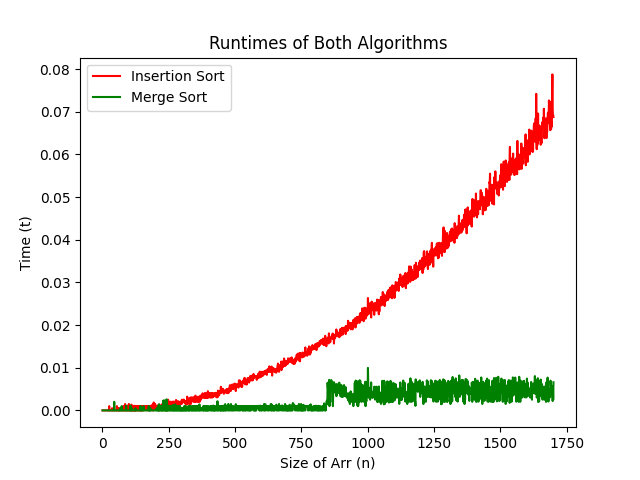
\includegraphics[width=0.9\textwidth]{images/runtime.png}
\caption{Runtime of Insertion Sort vs Merge Sort}
\label{fig:runtime}
\end{figure}    
As you can tell, around the $n=250$ mark, the merge sort algorithm starts to outperform the insertion sort algorithm. This is a simple problem which illustrates the practical benefits of recursion. Other interesting algorithms that use recursion include quicksort, heapsort, and many more. These algorithms are often more efficient than their iterative counterparts, and can be used to solve problems that are not efficiently solvable using loops.
\subsection{Other Examples of Algorithms that use Recursion}
There are many other examples of algorithms that use recursion, and I will not go into detail about all of them here. However, I will mention a few that are worth noting: \\
\begin{itemize}
    \item \textbf{Binary Search:} A classic algorithm that uses recursion to search for an element in a sorted array. The algorithm works by dividing the array into two halves, and searching for the element in the half that contains the element. The algorithm has a time complexity of \(\mathcal{O}(\log n)\).
    \item \textbf{Graph Algorithms:} Many graph algorithms use recursion to traverse graphs, such as depth-first search and breadth-first search. These algorithms are often more efficient than their iterative counterparts, and can be used to solve problems that are not efficiently solvable using loops.
    \item \textbf{Machine Learning Algorithms:} Many machine learning algorithms use recursion to optimize their parameters, such as gradient descent and backpropagation. These algorithms are often more efficient than their iterative counterparts, and can be used to solve problems that are not efficiently solvable using loops.
\end{itemize}
\section{Conclusion and further reading}
If any of you found the concept of recursion interesting, I would recommend you to read more about it. Due to the rigourous and complex nature of the subject, I will not be able to cover the mathematical intricacies in this article. However, I will recommend some resorces that you can use to learn more about these topics:
\begin{itemize}
    \item \textbf{Theory of Recursive Functions and Effective Computability} by Hartley Rogers: This is a classic book on the theory of recursive functions, and is a great resource for learning more about the subject. It covers the mathematical foundations of recursion, and provides a rigorous treatment of the subject.
    \item \textbf{Recursion Sequences} by Markushevich: This is a bite sized book and gives a lot of good insights and methods to solve problems using recursion. It is a great resource for learning more about the subject, and provides a lot of examples and exercises to help you understand the concepts better.
    \item \textbf{Binary, Hanoi and Sierpinski} by 3B1B: A fascinating video series that explores the concept of recursion and uses it to solve the Tower of Hanoi Problem.
\end{itemize}
Hope you enjoyed the article, cheers.
\end{document}
